% apdxa.tex

\chapter{MinBloq Programming Manual}\label{apdx:a}

\section{Hello World}

\textbf{Goal}: To display "Hello World" on the OLED display of the robot.

Click on the OLED display block. On clicking the red triangle to the right side of the block, a new pop-up expands which shows all the blocks related to display block. Click on the first block which is used to display a string. Click on the red triangle of the string block and select the last block "abc" which will help you type a string. Type "Hello World" as shown below. This completes the program to display "Hello World". Finally  port your program on to the robot. The program is shown in Figure~\ref{fig:lesson_1}

\begin{figure}[h]
\centering
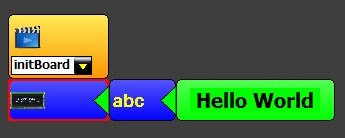
\includegraphics[width=0.35\columnwidth]{Images/Manual/lesson_1}
\caption{Program to display Hello World}
\label{fig:lesson_1}
\end{figure}

\section{Delays}

\textbf{Goal}: Blinking "Hello World" display.

Delay block pauses the program for the amount of time specified as parameter. There are two types of delay blocks - the millisecond delay block and the micro second delay block. Click on the millisecond delay block. Then click on the red arrow on the right hand side of the block that just appeared. Now, on the the second row of buttons that just popped up, click on the hash symbol . This is to send a constant value as a parameter. A box with a zero should have attached itself to the right side of the delay box. Type 1000 into it. This will tell the robot to wait one second (1000 ms)  before executing any other operations. The below program will blink the "Hello World" display 2 times with a delay of 1 second in between. Complete program is shown below in Figure~\ref{fig:lesson_2}

\begin{figure}[h]
\centering
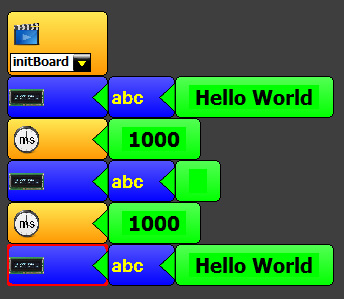
\includegraphics[width=0.6\columnwidth]{Images/Manual/lesson_2}
\caption{Program to demonstrate delays}
\label{fig:lesson_2}
\end{figure}

\section{Variables}

\textbf{Goal}: Pass the value for the delay block in previous program as a variable.

Variables are used when we want to store the data in the program. You can use them to hold values and then come back to them when you want to use that value. For example in the previous program, we have used 1000 ms for the delay block at two places. Instead of passing the value directly, we can store the value in a variable and then pass the variable to the delay block.

On the action window in Minibloq, there is a button that looks like a can. An empty can will define a new variable, and can only be used at the top of the program. A full can will reassign a variable's value. Click the empty can to initialize a new variable. Give it a name "delay". Assign a value 1000. Now in the previous program pass the delay variable for the delay block. Complete program is shown below in Figure~\ref{fig:lesson_3}

\begin{figure}[h]
\centering
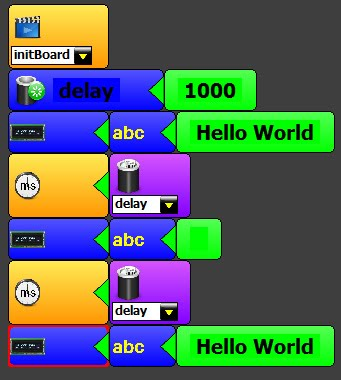
\includegraphics[width=0.4\columnwidth]{Images/Manual/lesson_3}
\caption{Program to demonstrate variables}
\label{fig:lesson_3}
\end{figure}

\section{If Statements}

\textbf{Goal}: Display "Hello World" if the value of a variable named "option" is 1 else display "Welcome".

An If statement allows the flow of the program to be changed, which leads to more interesting code. 

On the second row of the actions box, there is a "?" block. Click on that to implement an if statement. Three blocks should appear on your screen. The top indicates the start of the if. The second is the else. The bottom indicates the end of the if statement. Clicking on the red arrow on the right side of the top block will open up a boolean menu. If the expression evaluates to true, any blocks between it and the middle "if" block will execute. Otherwise any blocks between the middle and the bottom will execute. Click the equal to sign. This block can accept two values. Select the variable as one value and 1 in the other value as shown below. Complete program is shown below in Figure~\ref{fig:lesson_4}

\begin{figure}[h]
\centering
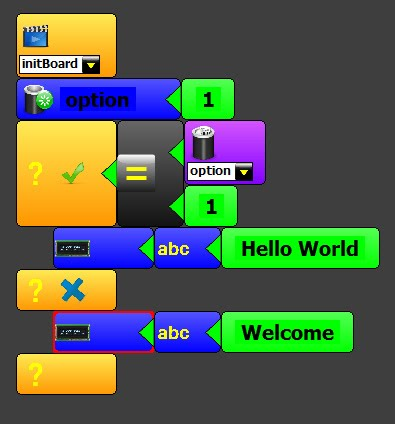
\includegraphics[width=0.4\columnwidth]{Images/Manual/lesson_4}
\caption{Program to demonstrate if statement}
\label{fig:lesson_4}
\end{figure}

\section{While loop}

\textbf{Goal}: Blinking "Hello World" continuously.

A while loop is a statement that allows code to be executed repeatedly based on a given boolean condition. The while construct consists of a block of statements and a condition. The condition is evaluated, and if the condition is true, the statements are executed. This repeats until the condition becomes false. 

On the actions window, there is a button on the upper left hand corner with a "?" and a cycle on it. This is a while loop block. Click on that to get two blocks on the screen. The top one receives a condition and everything between it and the bottom block executes as long as it is true. Click on the red arrow on the while block. Click on the Tick mark. It means the condition is true. Here we have created a never ending loop. This is necessary as we want the "Hello World" blinking continuously on the display. Complete program is shown below in Figure~\ref{fig:lesson_5}

\begin{figure}[h]
\centering
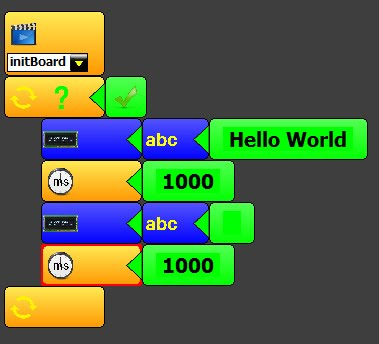
\includegraphics[width=0.5\columnwidth]{Images/Manual/lesson_5}
\caption{Program to demonstrate while loop}
\label{fig:lesson_5}
\end{figure}

\section{Repeat Loop}

\textbf{Goal}: To blink "Hello World" 10 times.

A repeat loop is a statement that allows code to be executed for given number of times. The repeat construct consists of a block of statements and a counter value. The counter value is incremented from zero for each block of execution. The statements are executed till the counter value is reached. 

On the actions window, there is a button on the upper right hand corner with a hash symbol and a circle on it. This is a repeat block. Click on that to get two blocks on the screen. The top one receives a counter value and everything between it and the bottom block executes till it counter value is reached. Click on the red arrow on the while block. Click on the hash symbol block to give counter a numeric value 10. Add blocks to blink "Hello World" between the two blocks for repeat. The complete program is shown below in Figure~\ref{fig:lesson_6}

\begin{figure}[h]
\centering
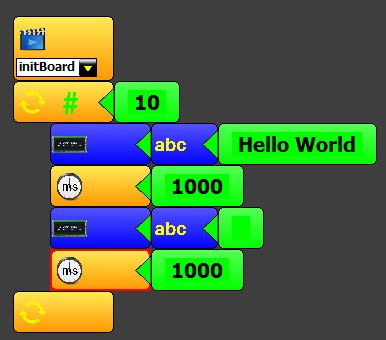
\includegraphics[width=0.5\columnwidth]{Images/Manual/lesson_6}
\caption{Program to demonstrate repeat loop}
\label{fig:lesson_6}
\end{figure}

\section{Movement}

\textbf{Goal}: To move the robot forward.

The movement block in the action window helps you to control the movement of the robot. This contains 5 blocks.
\begin{enumerate}
	\item Forward block
	\item Backward block
	\item Turn Left block
	\item Turn Right block
	\item Stop block
\end{enumerate}
To move the robot forward use the forward block. It takes in a parameter speed. Give a constant numeric value between 0 and 255. Add a delay block, to program for how much time the robot should move forward. If we give a value of 250, it means the robot keeps moving forward for 250 ms and then stops. Put the logic in a while loop so that, it keeps on moving forward every 250 ms. Complete program is shown below in Figure~\ref{fig:lesson_7}

\begin{figure}[h]
\centering
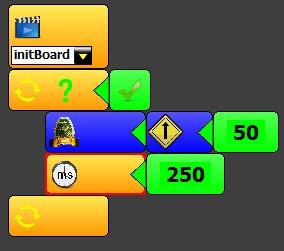
\includegraphics[width=0.25\columnwidth]{Images/Manual/lesson_7}
\caption{Program to demonstrate robot movement}
\label{fig:lesson_7}
\end{figure}

\section{Obstacle Sensor}

\textbf{Goal}: To stop the robot when it senses an obstacle ahead.

The obstacle sensor block, positioned in the number window, returns a numeric value (in cm) on how close the robot is to the obstacle. With this value you can set your own threshold, telling the robot on what to do when the threshold is reached. Check if the value returned by the obstacle sensor block is less than 20 cm. If yes, then stop the robot. Else keep moving forward. The complete program is shown below in Figure~\ref{fig:lesson_8}.

\begin{figure}[h]
\centering
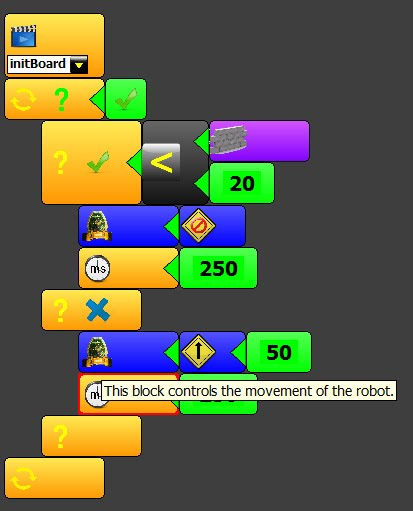
\includegraphics[width=0.6\columnwidth]{Images/Manual/lesson_8}
\caption{Program to demonstrate obstacle sensor}
\label{fig:lesson_8}
\end{figure}

\section{IR Sensor}

\textbf{Goal}: Make a floor tile black in color. When the robot enters the black tile, its speed decreases and when it comes out the tile, its speed returns back to normal.

IR sensors use Infra Red (IR) rays to emit and detect the amount of IR light that returns. Its usually used to detect between light and dark surfaces as light colored surfaces reflect more IR light than dark colored surfaces.

The IR sensor block is situated in the number window as it returns a number. Check if each sensor block is returning a value less than 50. That means its passing through a white tile. For white tiles, maintain a speed of 60 for the robot. If the value is greater than 50, its passing through a black tile. For black tiles, reduce the speed of the robot to 30.
Complete program is shown below in Figure~\ref{fig:lesson_9}.

\begin{figure}[h]
\centering
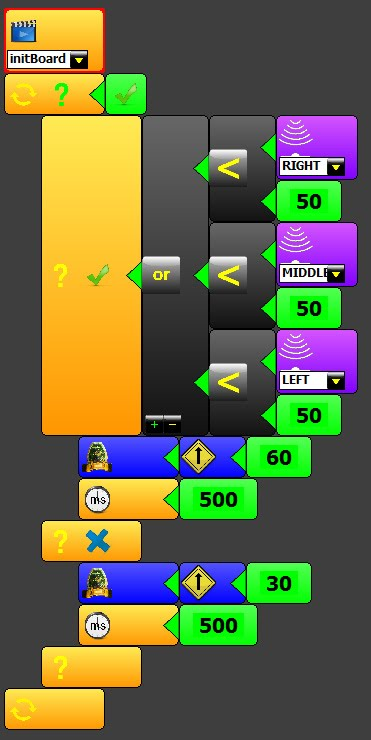
\includegraphics[width=0.3\columnwidth]{Images/Manual/lesson_9}
\caption{Program to demonstrate IR sensor}
\label{fig:lesson_9}
\end{figure}

\section{Buzzer}

\textbf{Goal}: To play the notes "c-d-e-f-g-a-b-c".

This lesson will help you use the buzzer to make musical notes. Before you start, make sure that the buzzer is activated with knob for the buzzer is in the right position. 

Click on the "Buzzer" block in the action bar. he block takes three parameters -

\begin{enumerate}
\item Note - Also referred as the pitch of the sound. This sets the frequency of the sound. By clicking on the red triangle button on the right of the block, user can select from 8 available frequencies (c, d, e, f, g, a, b, C). These are similar to the notes available in music.
\item Beat - This parameter sets the basic unit of time. For example, a note with beat "2" plays for a longer time than a note with a beat "1". Click on the red triangle button to get a number window pop-up. Select hash symbol to give a constant number 1 as input. 
\item Tempo - This sets the speed or pace of a given piece of music. So, if its a piece of music, its ideal to have the same tempo for all the notes. For the current task, set the value to a constant number "300". 
\end{enumerate}

Repeat the same steps for the notes d-e-f-g-a-b-C. Complete program is shown below in Figure~\ref{fig:lesson_10}. 

\begin{figure}[h]
\centering
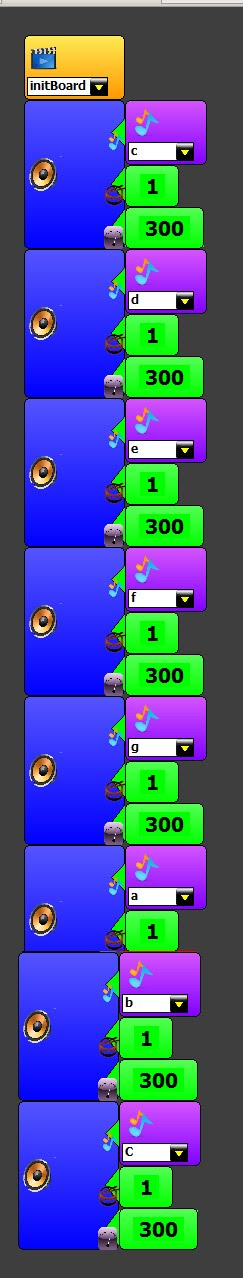
\includegraphics[width=0.25\columnwidth]{Images/Manual/lesson_10}
\caption{Program to demonstrate Buzzer}
\label{fig:lesson_10}
\end{figure}

